\documentclass[11pt]{article}

\usepackage{graphicx}
\usepackage[version=4]{mhchem}
\usepackage{lewis}
\usepackage{amsmath, expl3, calc}
\usepackage[utf8]{inputenc}

\setlength\parindent{0pt}

\title{CHEMISTRY 12 \\ J.L. Ilsley High School}
\author{Alyssa Motas}
\date{\today}

\begin{document}

    \maketitle

    \begin{center}
        \begin{tabular}{l r}
            Instructor: & Keri Butler
        \end{tabular}
    \end{center}

    \section{Thermochemistry}

    Thermochemistry is a field of study in chemistry where the heat energy is associated with chemical reactions and phase changes. The definition of energy is the capacity to do work.

    \begin{description}
        \item[radiant energy]
        comes from the sun and is earth's primary energy source 
        \item[thermal energy]
        is the energy associated with the random motion of atoms and molecules
        \item[chemical energy]
        is the energy stored within the bonds of chemical substances
        \item[nuclear energy]
        is the energy stored within the collection of neutrols and protons in the atom
        \item[potential energy]
        is the energy available by virtue of an object's position
        \item[kinetic energy]     
        is the energy due to motion
    \end{description}

    \subsection{Energy Changes in Chemical Reactions}
    \textbf{Heat} is the transfer of \textit{thermal energy} between two bodies that are at different temperatures. \textit{Temperature} is a measure of thermal energy, not the definition of itself. \\

    The \textit{system} is the specific part of the universe that is of interest in the study.

    \begin{description}
        \item[exothermic process]
        is any process that gives off heat--- transfers thermal energy from the system to the surroundings
        \item[endothermic process] is any process in which heat has to be supplied to the system from the surroundings
    \end{description}

    \subsection{More Definitions}

    \begin{description}
        \item[heat of fusion]
        the change in its enthalpy resulting from providing energy, typically heat, to a specific quantity of the substance to change its state from a solid to a liquid, at constant pressure
        \item[heat of formation]
        the heat released or absorbed (enthalpy change) during the formation of a pure substance from its elements at constant pressure (in their standard states)
        \item[heat of solution]
        the amount of heat energy that is released or absored when a solution is formed
        \item[calorimeter]
        a device that is used to measure the heat released or absorbed during a chemical or physical process occurring within it
        \item[heat of sublimination]
        the heat required to change one mole of a substance from solid  state to gaseous state at a give combination of temperature and pressure, usually standard temperatureand pressure (STP)
        \item[heat capacity]
        of a substance is the quantity of energy, in joules (J), required to change the temperature of the substance by one degree Celsius
        \item[first law of thermodynamics]
        energy can be converted from one form to another, but cannot be created or destroyed \\
        
        \begin{tabular}{ p{5cm} p{0.5cm} p{5cm} }
        Chemical energy \textbf{lost}  by combustion system & = & Energy \textbf{gained}  by the surroundings
        \end{tabular}

        \item[Enthalpy]
        is used to quantify the heat flow into or out of a system in a process that occurs at constant pressure

        \begin{center}
        $\Delta H = H_{products} - H_{reactants}$
        \end{center}

    \end{description}

    \subsection{Thermochemical Equations}
    The stoichiometric coefficients always refer to the number of moles of a substance.

    \begin{center}
        $\boxed{q = n\Delta H}$
    \end{center}

    \begin{center}
        \begin{tabular}{c l}
        $q$ & heat \\
        $n$ & moles \\
        $\Delta H$ & enthalpy
        \end{tabular}
    \end{center}

    \textbf{Example 1} What quantity of heat is required to melt 49g of \ce{H2O} at 0$^\circ$?

    \begin{center}
        \ce{H2O -> H2O} $\Delta H$ = 6.01 kJ

        \begin{equation*}
            q = \left(\text{49g \ce{H2O}} \times \frac{\text{1 mol}}{\text{18.02g \ce{H2O}}}\right) \left(\frac{\text{6.01 kJ}}{\text{1 mol \ce{H2O}}}\right) = \text{16.34 kJ}
        \end{equation*}
    \end{center}

    \textbf{Example 2} What mass of \ce{O2} was reacted if 2,000 kJ of heat was released?

    \begin{center}
        \begin{equation*}
            \begin{gathered}
                n = \frac{q}{\Delta H} = \frac{\text{-2,000 kJ}}{\frac{-890.4 \text{ kJ}}{1 \text{ mol \ce{O2}}}} = 4.5 \text{ mol \ce{O2}} \\
                \text{mass}_{\ce{O2}} = \left(4.5 \text{ mol \ce{O2}} \times \frac{32\text{g \ce{O2}}}{1 \text{ mol \ce{O2}}}\right) = 144\text{g \ce{O2}}
            \end{gathered}
        \end{equation*}
    \end{center}

    \begin{center}
        $\boxed{q = m C\Delta T}$

        \begin{tabular}{c l}
            $q$ & heat (kj/J)\\
            $m$ & mass (g) \\
            $C$ & specific heat capacity (J/g$^\circ$C) \\
            $\Delta T$ & change in temperature ($T_{f} - T_{i}$)
        \end{tabular}
    \end{center}

    Same substances have higher specific heat capacities than others. \\

    \textbf{Example 3} What amount of heat is released when 30g of \ce{Fe_{(s)}} cool from 70$^\circ$C to 25$^\circ$C? ($C_{Fe}$ = 0.444 J/g$^\circ$C)

    \begin{equation*}
        q = (30\text{g})(0.444 \text{J/g}^\circ \text{C})(25^\circ \text{C} - 70^\circ \text{C}) = -599.4 \text{J} \leftarrow \text{exothermic}
    \end{equation*}

    \newpage
    \subsection{Phase Changes - Water and Energy}

    \begin{figure}[h]
        \begin{center}
        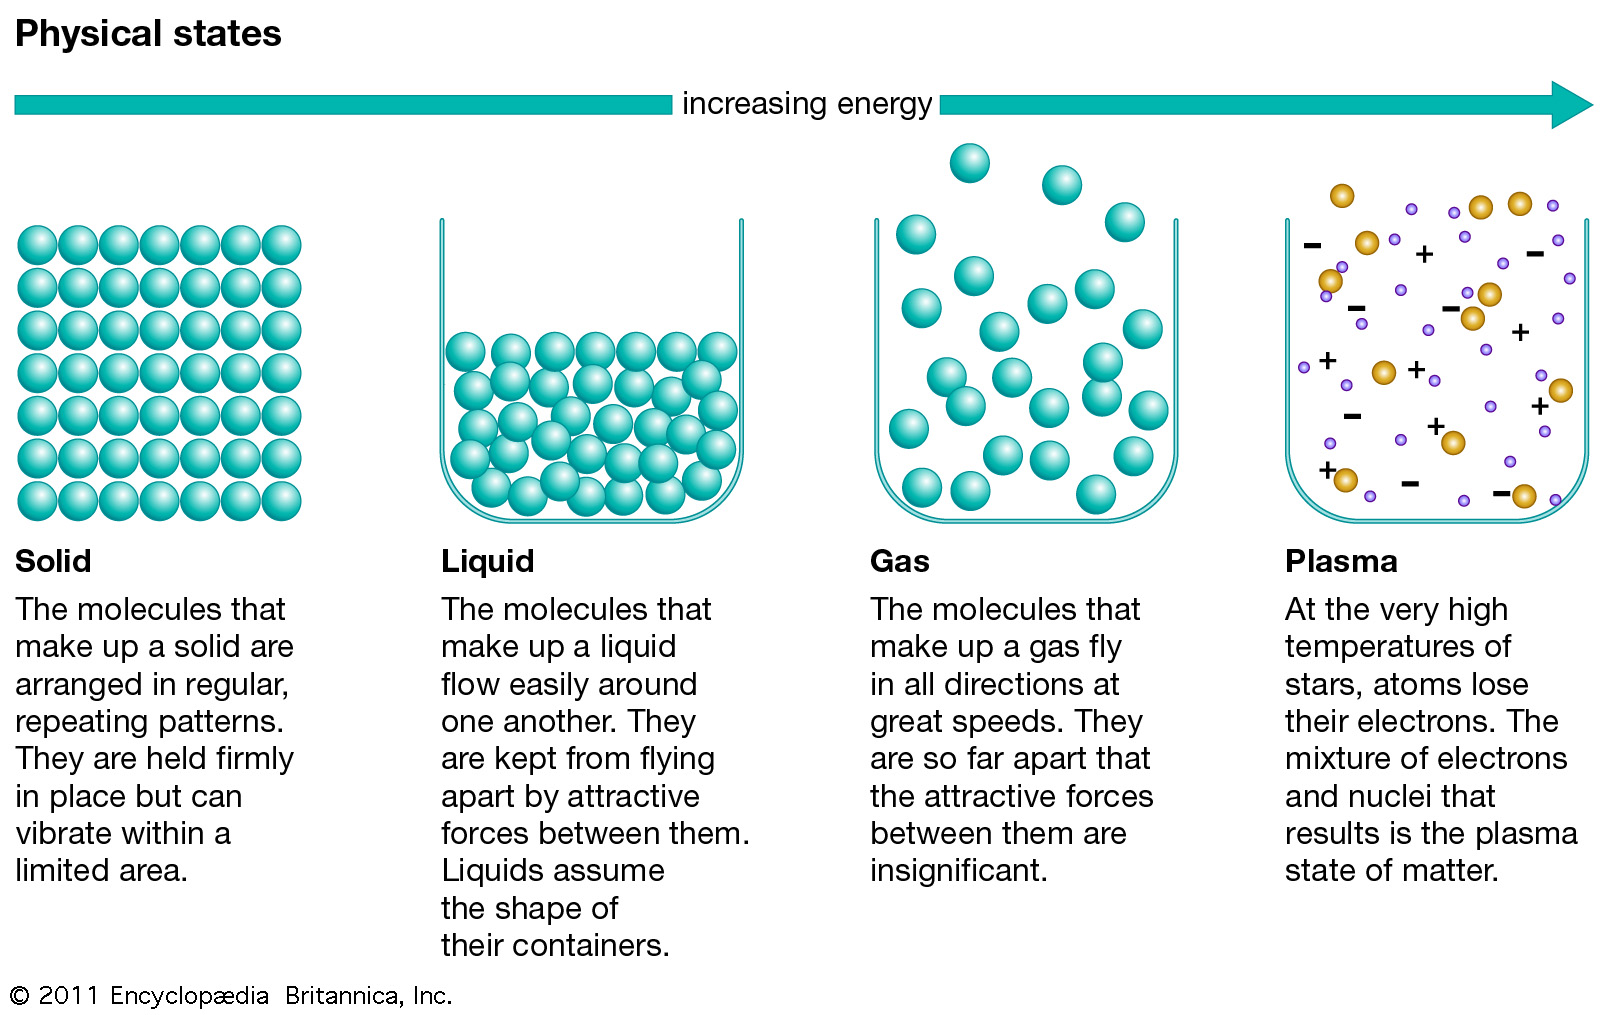
\includegraphics[width=10cm]{States-matter}
        \caption{States of Matter}
        \end{center}
    \end{figure}
    \begin{figure}[h]
        \begin{center}
        \includegraphics[width=7cm]{Phase_change}
        \caption{Phase Change Graph of Water}
        \end{center}
    \end{figure}

    \begin{center}
        ice $\rightarrow$ water $\rightarrow$ steam

        \begin{tabular}{c l}
            $\uparrow$ & $q=mc\Delta T$ \\
            $\rightarrow$ & $q=n\Delta H$
        \end{tabular}

        $\Delta H_{vaporization}$ = 40.7 kJ/mol \\
        $\Delta H_{fusion}$ = 6.02 kJ/mol
    \end{center}

    \subsection{Types of Phase Change Calculations}
    \begin{description}
        \item[One step (Melting/Freezing or Vap/Condense)] at 0$^\circ$C or 100$^\circ$C (for water)
        \item[Multi-step] use the heating/cooling curves for calculations (max 3 steps)
        \item[Problem solving] for mass or final temperature 
    \end{description}

    \textbf{Example 1} What amount of heat is needed to melt 150g of ice at 0$^\circ$C?

    \begin{equation*}
        \begin{aligned}
            q&=n\Delta H \\
            &= \left(150\text{g} \times \frac{1 \text{ mol}}{18.02 \text{g}}\right)\left(\frac{6.02\text{ kJ}}{1 \text{ mol}}\right) \\
            q&=50.11 \text{ kJ}
        \end{aligned}
    \end{equation*}

    \textbf{Example 2} What amount of heat is released when 40g of steam at 110$^\circ$C is condensed to liquid at 100$^\circ$C?

    \begin{equation*}
        \begin{aligned}
            q_{1} + q_{2} &= q_{total} \\
            q_{1} &= (40\text{g})(2.01\text{ J/g}^\circ\text{C})(100^\circ\text{C} - 110^\circ\text{C}) \\
            &=-804 \text{ J} \times \frac{1\text{ kJ}}{1,000 \text{ J}} \\
            q_{1} &= -0.804\text{ kJ}\\
            q_{2} &= \left(40\text{g} \times \frac{1\text{ mol}}{18.02\text{g}}\right)\left(\frac{-40.7\text{ kJ}}{1 \text{ mol}}\right) \\
            &= -90.34 \text{ kJ} \\
            q_{total} &= -0.804\text{ kJ} + -90.34 \text{ kJ} \\
            &= -91.14 \text{ kJ}
        \end{aligned}
    \end{equation*}

    \subsection{Heats of Chemical Reactions}
    \begin{description}
        \item 1. Using heats (enthalpies) of formation
        \item 2. Using Hess' Law
        \item 3. Using bond energies
    \end{description}
    \newpage

    \subsubsection{Enthalpies of Formation}
    If 1 mol of compound is formed from its constituent elements, then the enthalpy change for the reaction is called the \textbf{enthalpy of formation, $\Delta H^\circ_{f}$}. \\
    \\
    Standard condition/state -  Most stable form of the substance at 1 atm (atmospheric pressure) and 25$^\circ$C (298 K). \\
    \\
    Standard enthalphy, $\Delta H^\circ$, is the enthalpy measured when everything is in its standard state. \\
    \\
    Standard enthalphy of formation - 1 mol of compound is formed from substances in their standard states. These values are found in a data table. If there is more than one state for a substance under standard conditions, the more stable one is used. The value of these stable elements (HOBrFINKL) is zero.

    \begin{equation*}
        \boxed{\Delta H^\circ_{rxn} = \sum n \cdot \Delta H^\circ_{f (products)} - \sum m \cdot \Delta H^\circ_{f (reactants)} }
    \end{equation*}
    \\
    \textbf{Example} Calculate the heat of reaction for the combustion of propane gas giving carbon dioxide and water.

    \begin{center}
        \ce{C3H8_{(g)} + 5 O2_{(g)} -> 3 CO2_{(g)} + 4 H2O_{(g)}}
    \end{center}

    \begin{equation*}
        \begin{aligned}
            \Delta H_{f (products)} &= \ce{3 CO2_{(g)} + 4 H2O_{(g)}} \\
                                    &= 3 \text{ mol} \times \frac{-393.5 \text{ kJ}}{1 \text{ mol}} + 4 \text{ mol} \times \frac{-241.8 \text{ kJ}}{1 \text{ mol}} \\
                                    &= -2147.7 \text{ kJ} \\
            \Delta H_{f (reactants)}&= \ce{C3H8_{(g)} + 5 O2_{(g)}} \\
                                    &= 1 \text{ mol} \times \frac{-103.8 \text{ kJ}}{1 \text{ mol}} \\
                                    &= -103.8 \text{ kJ} \\
            \Delta H_{rxn}          &= -2147.7 \text{ kJ} - (-103.8 \text{ kJ}) \\
                                    &= -2043.9 \text{ kJ} \leftarrow \text{exothermic}
        \end{aligned}
    \end{equation*}

    Note: \ce{H2O} can be liquid or vapour and they have different $\Delta H_{f}$.

    \newpage
    \subsubsection{Hess' Law}

    If a reaction is carried out in a number of steps, $\Delta H$ for the overall reaction is the sum of $\Delta H$ for each individual step. \\
    \\
    Equations can be manipulated to form the overall reaction (multiply by a coefficient, flip the reaction by a negative number). \\
    \\
    \textbf{Example} Determine the heat of reaction for the reaction:
    \begin{center}
        \ce{4 NH3_{(g)} + 5 O2_{(g)} -> 4 NO_{(g)} + 6 H2O_{(g)}}
    \end{center}

    Using the following sets of reactions:
    \begin{center}
        \begin{tabular}{l l}
            (1) \ce{N2_{(g)} + O2_{(g)} -> 2 NO_{(g)}}      & $\Delta H$ = 180.6 kJ \\
            (2) \ce{ N2_{(g)} + 3 H2_{(g)} -> 2 NH3_{(g)} } & $\Delta H$ = -91.8 kJ \\
            (3) \ce{ 2 H2_{(g)} + O2_{(g)} -> 2 H2O_{(g)} } & $\Delta H$ = -483.7 kJ \\
        \end{tabular} 
        \break
        \\
        Steps to do:      (1) $\rightarrow \times 2$,
                (2) $\rightarrow \times -2$,
                 and (3) $\rightarrow \times 3$ 
    \end{center}

    \begin{center}
        \begin{tabular}{l l}
            (1) 2 $\times \left(\ce{N2_{(g)} + O2_{(g)} -> 2 NO_{(g)}}\right)$      & 2 $\times \left(\Delta H = 180.6 \text{ kJ}\right)$ \\
            (2) -2 $\times \left(\ce{ N2_{(g)} + 3 H2_{(g)} -> 2 NH3_{(g)} }\right)$ & 2 $\times \left(\Delta H = -91.8 \text{ kJ}\right)$ \\
            (3) 3 $\times \left(\ce{ 2 H2_{(g)} + O2_{(g)} -> 2 H2O_{(g)} }\right)$ & 2 $\times \left(\Delta H = -483.7 \text{ kJ}\right)$ \\
        \end{tabular}

        \noindent\rule{11cm}{0.4pt}
        \begin{tabular}{l l}
            (4) \ce{ 4 NH3 + 5 O2 -> 4 NO + 6 H2) } & $\Delta H_{rxn}$ = -906.3 kJ
        \end{tabular}
    \end{center}

    \subsubsection{Bond Energies}
    Breaking bonds is an endothermic process (positive), while bonds forming is an exothermic process (negative). There is an energy value for a specific bond, usually measured in kJ/mol. The formula to find the heat of reaction is $\Delta H_{rxn} = \text{BB (Bonds Broken)} - \text{BF (Bonds Formed)}$. \\
    \\
    \textbf{Example} Determine the $\Delta H_{rxn}$ using bond energies:

    \begin{center}
        \ce{ 2 C2H6 + 7 O2 -> 4 CO2 + 6 H2) } \\
        \break
        \begin{tabular}{ c | c }
            Bonds Broken & Bonds Formed \\
            2 (1 C-C + 6 C-H) + 7 (O=O)& 4(2 C=O) \\
        \end{tabular}
    \end{center}

    \begin{center}
        Let $\alpha$ = Bonds Broken \\
            $\beta$ = Bonds Formed \\
    \end{center}

    \begin{equation*}
        \begin{aligned}
            \alpha          &= \left(2 \text{ mol} \times \frac{348 \text{ kJ}}{1 \text{ mol}} \right) + \left(12 \text{ mol} \times \frac{413 \text{ kJ}}{1 \text{ mol}}\right) + \left(7 \text{ mol} \times \frac{495 \text{ kJ}}{1 \text{ mol}}\right) \\
                            &= 9117 \text{ kJ} \\
            \beta           &= \left(8 \text{ mol} \times \frac{799 \text{ kJ}}{1 \text{ mol}}\right) + \left(12 \text{ mol} \times \frac{463 \text{ kJ}}{1 \text{ mol}}\right) \\
                            &= 11 948 \text{ kJ} \\
            \Delta H_{rxn}  &= \alpha - \beta \\
                            &= 9117 \text{ kJ} - 11948 \text{ kJ} \\
                            &= -2831 \text{ kJ}
        \end{aligned}
    \end{equation*}

    \section{Solutions}

    \subsection{Definitions}

    \begin{description}
        \item[solution] a homogeneous mixture
        \item[solute] substance being dissolved
        \item[solvent] the component present in the greatest amount
        \item[aqueous solution] solution which has water for the solvent
        \item[] e.g. salt is the \emph{solute} and water is the \emph{solvent} 
        \item[concentrated solution] higher proportion of solute to solvent than a diluted solution
        \item[diluted solution] has a lower proportion of solute to solvent than a concentrated solution
        \item[solvation] the process of dissolving (the process i which an ion or molecule is surrounded by solvent molecules arranged in a specific manner)  
        \item[]e.g. solvent-solvent, solute-solute, and solvent-solute interactions
        \item[electrolyte] is a substance that, when dissolved in water, gives a solution that can conduct electricity
        \item[non-electrolyte] does not conduct electricity when dissolved in water
        \item[solubility] the amount of solute that can be dissolved in a given amount of a saturated solution at a fixed temperature is the \emph{solubility} of the solute in the solvent
        \item[]e.g. unsaturated (more solute), saturated (more than enough), and supersatured (crystals form) solution
        \item[solubility curve] shows the dependence of solubility on temperature; x (temperature) and y (grams solute per 100mL water)
        \item[]Note: Anything that falls below the line is \emph{unsaturated}, otherwise it's \emph{supersaturated}
        \item[solids] more soluble at higher temperatures
        \item[gases] more soluble at low temperatures and high pressures
        \item[miscible] liquids that are soluble in each other
        \item[immiscible] liquids that do not mix together
    \end{description}

    \subsection{Concentration Calculations}
    1. mass-mass \% \\
    2. volume-volume \% \\
    3. mass-volume \% \\
    4. parts per million/billion

    \subsubsection{mass-mass \%}

    \begin{equation*}
        m/m \% = \frac{\text{mass of solute(g)}}{\text{mass of solution (g)}} \times 100 \%
    \end{equation*}

    \textbf{Example} An alloy of 2.7g \emph{gold} jewelry is 83\% pure gold. What mass of gold is in the jewelry?
    \begin{equation*}
        \begin{aligned}
            m/m \% &= \frac{\text{mass of solute(g)}}{\text{mass of solution (g)}} \times 100 \% \\
            83 \% &= \frac{x}{2.7\text{g}} \times 100 \% \\
            0.83 &= \frac{x}{2.7\text{g}} \\
            x &= 2.24\text{g}
        \end{aligned}
    \end{equation*}

    \subsubsection{volume-volume \%}

    \begin{equation*}
        v/v \% = \frac{\text{volume of solute (mL)}}{\text{volume of solution (mL)}} \times 100 \%
    \end{equation*}

    \textbf{Example} A 53mL sample of \ce{H2O2} is dissolved in enough water to make 250mL of solution. Determine the v/v \% of \ce{H2O2}.

    \begin{equation*}
        v/v \% = \frac{53\text{mL}}{250\text{mL}} \times 100 \% = 21.2 \%
    \end{equation*}

    \subsubsection{mass-volume \%}

    \begin{equation*}
        m/v \% = \frac{\text{mass of solute (g)}}{\text{volume of solution (mL)}} \times 100 \%
    \end{equation*}

    \textbf{Example} Determine the mass/volume \% of \ce{NaCl} if 30g of salt is dissolved in 500mL of water. Assume no change in volume.

    \begin{equation*}
        m/v \% = \frac{30\text{g}}{500\text{mL}} \times 100 \% = 6 \%
    \end{equation*}

    \subsubsection{parts per million/billion}

    \begin{equation*}
        \begin{aligned}
        ppm &= \frac{\text{mass of solute (g)}}{\text{mass of solution (g)}} \times 10^6 \\
        ppb &= \frac{\text{mass of solute (g)}}{\text{mass of solution (g)}} \times 10^9
        \end{aligned}
    \end{equation*}

    \textbf{Example} Determine the \emph{ppm} of \ce{Fe^{2+}} if 3.5mg is dissolved in a 100g sample of water.

    \begin{equation*}
        ppm = \frac{0.0035\text{g}}{100\text{g}} \times 10^6 = 35 ppm
    \end{equation*}

    \subsection{Molarity}
    This describes the mols of solute per litre of solution. The unit is mol/L or M.

    \begin{equation*}
        \boxed{M = \frac{n}{V}}
    \end{equation*}

    \begin{center}
        \begin{tabular}{c l}
            $M$ & molarity of the solution \\
            $n$ & number of mols \\
            $V$ & volume (L) \\   
        \end{tabular}
    \end{center}

    \textbf{Types of questions} \\
    1. solving for molarity \\
    2. solving for mass \\
    3. solving for volume

    \subsection{Dilution}

    \begin{equation*}
        M_{1}V_{1} = M_{2}V{2}
    \end{equation*}

    \begin{center}
        \begin{tabular}{c l}
            $M_{1}$ & molarity of solution 1 \\
            $V_{1}$ & volume of solution 1 \\
            $M_{2}$ & molarity of solution 2 \\
            $V_{2}$ & volume of solution 2
        \end{tabular}
    \end{center}

    \subsubsection{Preparing Solutions}
    Weigh out a solid solute and dissolve in a given quantity of solvent. (Solid Solute). \\
    Dilute a concentrated solution to give one that is less concentrated. (Liquid) \\
    \break
    \textbf{Steps: (Solid)} \\
    1. Calculate the mass of solute required. Weigh out sample on a balance. \\
    2. Dissolve solid in some water in a beaker. \\
    3. Transfer to a volumetric flask. \\
    4. Bring to volume with water.\\
    \break
    \textbf{Steps: (Liquid)} \\
    1. Calculate the volume of solute required. Measure using a pipet. \\
    2. Add solute to water in the volumetric flask. \\
    3. Bring to volume with water.

    \subsection{Solubility Rules and Precipitation Reactions}
    Not all ionic compounds dissolve! Instead of doing experiments all the time to see which ones will dissolve, we use the \emph{solubility rules}.

    \subsubsection{General Solubility Rules}
    1. All nitrates (\ce{NO3^{-}}) are \emph{soluble}. \\
    2. All ammomium (\ce{NH4^{+}}) or alkali (\ce{Li^{+}, Na^{+}, K^{+}, Rb^{+}, Cs^{+}, Fr^{+}}) compounds are \emph{soluble}. \\
    3. All carbonates (\ce{CO3^{2-}}), phosphates (\ce{PO4^{3-}}) and hydroxides (\ce{OH^{-}}) are \emph{insoluble} \textbf{except} with the cations in rule 2. \\
    4. All chlorides (\ce{Cl^{-}}), bromides (\ce{Br^{-}}), and iodides (\ce{I^{-}}) are \emph{soluble} \textbf{except} with \ce{Ag^{+}, Pb^{2+}, Hg^{+}}. \\
    5. All sulfates (\ce{SO4^{-2}}) are \emph{soluble} \textbf{except} with \ce{Ca^{2+}, Sr^{2+}, Ba^{2+}, Ra^{2+}, Pb^{2+}}.
    6. All acetates are \emph{soluble} (\ce{CH3COO^{-}, C2H3O2^{-}}).

    \subsubsection{Precipitation Reactions}
    A reaction that produces an insoluble salt is precipitation reaction. The insoluble substance is called a precipitate (ppte). Reactions that form a precipitate have a net ionic equation that shows the ions involved in forming the percipitate. \\

    \textbf{Example} \ce{Na2SO4_{(aq)} + Ca(NO3)2_{(aq)} -> 2 NaNO3_{(aq)} + CaSO4_{(s)}}
    \begin{center}
        \ce{NaNo3} = soluble \\
        $\boxed{\ce{CaSo4} = \text{insoluble}}$
    \end{center}

    \begin{center}
        $\underbrace{\ce{2 Na^{+} + SO4^{-2} + Ca^{+2} + 2 NO3^{-} -> 2 Na^{+} + 2 NO3^{-} + CaSO4_{(s)}}}_\text{Total ionic equation}$
        $\underbrace{\ce{Ca^{+2} + SO4^{-2} -> CaSO4_{(s)}}}_\text{Net ionic equation}$
    \end{center}

    \subsection{Aqueous Reactions and Solution Stoichiometry}
    The majority of work in research and industry involves solutions. Solutions are easy to handle and are usually easier to control in reactions. Solution stoichiometry is the procedure for calculating the molar concentration or volume of solution products or reactants.

    \textbf{Types of Problems} \\
    1. Unknown Volume \\
    2. Unknown Molarity \\
    3. Mass (of precipitate usually) \\

    \textbf{Example} Ammonia and phosphoric acid solutions are used to produce ammonium hydrogen phosphate fertilizer. What volume of 14.8M \ce{NH3_{(aq)}} is needed to react with 1000L of 12.9M of \ce{H3PO4_{(aq)}}?

    \begin{center}
        \ce{2 NH3_{(aq)} + H3PO4_{(aq)} -> (NH4)2HPO4_{(aq)}}
    \end{center}

    \begin{equation*}
        1000 \text{L} \times \frac{12.9 \text{mol}}{1 \text{L}} \times \frac{2 \text{ mol}}{1 \text{ mol}} \div 14.8 \text{ mol/L} = 1740\text{L}
    \end{equation*}

    \subsection{Qualitative Analysis}
    What is qualitative chemical analysis? it is a branch of chemistry that deals with the identification of elmeents or grouping of elements present in a sample. There are usually two types: \emph{qualitative inorganic analysis} and \emph{qualitative organic analysis}.

    \subsubsection{Identifying Ions}
    Chemists often have to determine what substances (ions) are in mixtures with no information. They can use solubility rules (or chart) to determine solubility when solutions contain unknown ions. To create a procedure, we'll need to look at what tests we can do to "figure it out". \\
    \newpage
    \textbf{Flow Chart Example} \\

    $\ce{K^{+}/Ag^{+}} \rightarrow \text{add } \ce{Cl^{-}} \rightarrow \text{ppte} \rightarrow \ce{Ag^{+}} \text{ present, filter it out} \rightarrow \text{flame test} \rightarrow \text{lilac means \ce{K^{+}}} \text{ present} $

    If no ppte, \ce{Ag^{+}} is not present.

    \section{Kinetics and Equilibrium}

    What is chemical kinetics? Kinetics is the study of reaction rates. A rate involves a change in a variable over a change in time.

    \begin{equation*}
        \begin{aligned}
            \text{average rxn rate} &= \frac{\text{change in the number of mols of $\beta$}}{\text{change in time}} \\
                                    &= \frac{\Delta \text{(moles of $\beta$)}}{\Delta T} \\
                                    &= \frac{-\Delta \text{moles of $\alpha$}}{\Delta T}
        \end{aligned}
    \end{equation*}

    How to measure the rate of reaction? Two ways: measure how quickly one of the products is \emph{made}, or measure how quickly one of the reactants \emph{disappears}.

    \textbf{Example} A student reacts Mg with HCl, and obtained the following data about the mass of Mg that reacted.

    \begin{center}
        \begin{tabular}{| r | r |}
            \hline
            Time(s) & Mass(g) \\ \hline
            0 & 1.5 \\
            5 & 1.2 \\
            10 & 0.9 \\
            15 & 0.6 \\
            20 & 0.3 \\ \hline
        \end{tabular}
    \end{center}

    a) Determine the rate of reaction (in g/s) between 10 and 20 seconds. \\
    
    \begin{equation*}
        \text{rate}_{10 \rightarrow 20} = \frac{0.3-0.9}{20-10} = -0.06\textbf{g/s}
    \end{equation*}

    b) Determine the rate of reaction between 0 and 20 seconds in mol/s.

    \begin{equation*}
        \text{rate} = \frac{0.3-1.5}{20-0} = \frac{-1.2}{20} = -0.06\text{g/s} \times \frac{1 \text{ mol}}{24.31\text{g}} = -0.00247 \text{ mol/s}
    \end{equation*}

    \subsection{Instantaneous Rate vs Average Rate of Rxn}
    Instantaneous rate is the rate at that \emph{exact} time (slope of the tangent line). The average rate is $\frac{\Delta \text{quantity}}{\Delta \text{time}} = $ slope. \\

    \textbf{Example} \\
    \begin{center}
        \ce{N2 + 3 H2 -> 2 NH3} \\
        rate of appearance of \ce{NH3} = 2.0 x 10$^{-3}$ M/s \\
    \end{center}

    a) What is the rate of disappearance of \ce{N2}?

    \begin{equation*}
        \begin{aligned}
            \text{rate}_{\ce{ N2}} &= -\left(2.0 \times 10^{-3} \text{ M/s} \times \frac{1 \ce{ N2}}{2 \ce{ NH3}}\right) \\
            &= -1 \times 10^{-3} \text{ M/s \ce{NH3}}
        \end{aligned}
    \end{equation*}

    \subsection{Kinetic Molecular Theory}
    1. All matter is made up of \emph{microscopic-sized particles} (atoms, molecules, ions). \\
    2. These particles are in constant motion because they possess \emph{kinetic energy}. \\
    3. There are spaces between the partciles of matter. The speed and spacing determine the \emph{physical state} of matter. \\
    4. Adding heat increases the speed of the moving particles, thus increasing their kinetic energy as well as the space they occupy.

    \subsection{Collision Theory}
    The collision transfers kinetic enregy needed to break the necessary bonds so that new bonds can be formed.\\
    1. In order for a chemical reaction to take place, the reactants must \emph{collide}. \\
    2. They must have \emph{proper orientation}. \\
    3. Must have enough kinetic enregy to reach a threshold of enregy called \emph{activation energy}. \\
    
    \subsection{Factors Affecting The Rate of Reaction}
    What needs to happen in order for the rate of the chemical reaction to increase (go faster)?

    \begin{center}
        More collisions = Faster reaction rate
    \end{center}

    \begin{description}
        \item[Nature of reactants] how reactive they are; ionic vs. covalent
        \item[Concentrations of reactants] generally speaking, the higher the concentration of reactants, the faster the rate of the reaction
        \item[Temperature] the higher the temperature, the fsater the rate of reaction
        \item[The presence of a catalyst] a catalyst is able to increase the rate of reaction, although the catalyst itself is neither created nor destroyed when performing this function; catalysts don't \emph{cause} a reaction, they just speed it up (lower the activation energy)
        \item[The surface area of the reactants or catalysts] reactions that involve solids often proceed faster if the solid is a fine powder instead of big chunky bits; the physical difference of the two is the surface area
        \item[pressure] gases only; gases tend to expand, making collisions less frequen; increasing pressure (by reducing volume) allows for more collisions to occur
        \item[light] solar energy can act as a catalyst
        \item[agitation] stirring, shaking; allows particles to increase speed and collide with each other        
    \end{description}

    \subsection{Potential Energy Diagrams}

    \begin{figure}[h]
        \begin{center}
        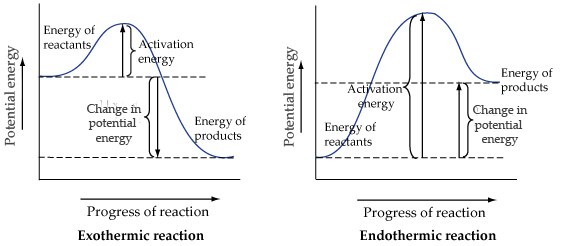
\includegraphics[width=10cm]{pe_diagram}
        \caption{Potential Energy Diagrams}
        \end{center}
    \end{figure}

    \begin{description}
        \item[activation energy, $E_{a(forward)}$] the amount of enregy required to reach the transition state or activated complex from the reactants; the reverse is from products to the transition state
        \item[transition state/activated complex] when bonds break and form and reactants become products 
    \end{description}

    \subsection{Reaction Mechanisms}
    The sequence of events that describes the actual process by which reactants become products is called the reaction mechanism. Each of these processes is known as an elementary reaction or process. Molecules, atoms, or ions that are formed during these steps are called reaction intermediates. \\
    \break
    To get the overall balanced equation from a proposed mechanism, you must add the elementary reactions together, then cancel out the species that show up on both sides of the reaction. \\
    \break
    The molecularity refers to the number of reactant particles that are involved in an elementary reaction.
    
    \begin{center}
        \begin{tabular}{| l | r |}
            \hline
            Molecularity & Elementary Reaction \\ \hline
            Unimolecular & $\alpha \rightarrow$ products \\
            Bimolecular & $\alpha + \beta \rightarrow$ products \\
            Termolecular & $\alpha + \beta + \lambda \rightarrow$ products \\ \hline
        \end{tabular}
    \end{center}

    The overall reaction speed cannot move faster than the slowest step, known as the rate-determining step.

    \begin{center}
        \begin{tabular}{c c}
            Intermediate & Catalyst \\
            P $\rightarrow$ R & R $\rightarrow$ P
        \end{tabular}
    \end{center}

    \subsection{Rate Laws}
    The rate law expresses the relationship of the rate of rxn to the rate constant and the concentrations of the reactants to some powers.

    \begin{center}
        aA + bB $\rightarrow$ cC + dD \\
        Rate = k[A]$^{x}$[B]$^{y}$ \\
        Rxn is x$^{th}$ order in A \\
        Rxn is y$^{th}$ order in B \\
        Rxn is (x + y)$^{th}$ order overall \\
        \break
        k = rate constant \\
        e.g. k = $\frac{\text{rate}}{[\ce{F2}][\ce{ClO2}]}$
    \end{center}

    \subsection{Chemical Equilibrium}
    Equilibrium reactions are reversible and only happens in a closed system.

    \begin{equation*}
        \begin{gathered}
            K_{c} = \frac{[C]^{c}[D]^{d}}{[A]^{a}[B]^{b}} \\
            K_{c} = \frac{products}{reactants} 
        \end{gathered}
    \end{equation*}

    \begin{center}
        Note: no solids and pure liquids allowed
    \end{center}

    \subsubsection{$K_{c}$ Values}

    \begin{center}
        \begin{tabular}{ | r | c |}
            \hline
            K $>$ 1 & products dominate EQ \\ \hline
            K $<$ 1 & reactants dominate EQ \\ \hline
            K = 1 & products and reactants are equal \\ \hline
        \end{tabular}
    \end{center}

    \textbf{Types of Problems} \\
    1. Plug-n-Chug \\
    2. Algebra (ICE table) \\
    3. Percent Reaction (ICE table) \\
    4. Perfect Square (ICE table)

    \subsection{Predicting Shifts in Equilibrium}
    \subsubsection{Reaction Quotient}

    \begin{equation*}
        Q = \frac{[C]_{i}[D]_{i}}{[A]_{i}[B]_{i}}
    \end{equation*}

    \begin{center}
        Q $<$ K, not enough products (shift right) \\
        Q = K, system is at EQ \\
        Q $>$ K, not enough reactants
    \end{center}

    \subsubsection{Le Ch\^atelier's Principle}
    If a stress is applied to a system at EQ, the system will change to relieve that stress and re-establish equilibrium. \\

    \textbf{Factors that Affect EQ} \\
    1. Concentration 
    \begin{center}
        Add more reactant $\rightarrow$ Shift right \\
        Remove reactants $\rightarrow$ Shift left \\
        Add more product $\rightarrow$ Shift left \\
        Remove products $\rightarrow$ Shift right
    \end{center}
    2.1. Temperature Change: Exothermic Rxn \\
    - Consider heat as a \emph{product}
    \begin{center}
        Add heat $\rightarrow$ shift left (K decreases)
        Remove heat $\rightarrow$ shift right (K increases)
    \end{center}
    2.2. Temperature Change: Endothermic Rxn \\
     - Consider heat as a \emph{reactant}
    \begin{center}
        Add heat $\rightarrow$ shift right (K increases) \\
        Remove heat $\rightarrow$ shift left (K decreases)
    \end{center}
    3. Pressure Changes \\
    - Only affects systems with \emph{unequal} moles of gaseous reactants and products.
    \begin{center}
        Increase pressure $\rightarrow$ shifts to the less molecule(s) \\
        Decrease pressure $\rightarrow$ shifts to more molecule(s)
    \end{center}
    4. Presence of a Catalyst \\
    - Only speeds up the rate of reaction \\
    5. Presence of an Inert Substance \\
    - An inert substance is not reactive with any species and will not affect the system

    \section{Acids and Bases}

    \begin{center}
        \begin{tabular}{ | p{5cm} | p{5cm} | }
            \hline
            Acids & Bases \\ \hline
            $\rightarrow$ Have a sour taste & $\rightarrow$ Have a bitter taste \\
            $\rightarrow$ Reacts with certain metals to produce hydrogen gas & $\rightarrow$ Feels slippery \\
            $\rightarrow$ Reacts with carbonates/bicarbonates to produce carbon dioxide gas & $\rightarrow$ pH greater than 7 \\
            $\rightarrow$ pH less than 7 & $\rightarrow$ Turns red litmus blue \\
            $\rightarrow$ Turns blue litmus red & $\rightarrow$ Conducts electricity \\
            $\rightarrow$ Conducts electricity & $\rightarrow$ Changes colour with an indicator \\
            $\rightarrow$ Changes colour in indicators & $\rightarrow$ Reacts with acids in a neautralization to produce a salt and water \\ \hline
        \end{tabular}
    \end{center}

    \subsection{Acid-Base Theories}
    \subsubsection{Arrhenius Acids}
    An Arrhenius acid is a substance that produces \ce{H^{+}} (\ce{H3O^{+}}) in water.

    \begin{center}
        \ce{HCl_{(g)} + H2O_{(l)} -> H3O^{+}_{(aq)} + Cl^{-}_{(aq)}}
    \end{center}

    \subsubsection{Arrhenius Bases}
    An Arrhenius base is a substance that produces \ce{OH^{-}} in water.

    \begin{center}
        \ce{NaOH_{(s)} -> Na^{+}_{(aq)} + OH^{-}_{(aq)}}
    \end{center}

    \subsubsection{Br\o nsted-Lowry}
    A Br\o nsted-Lowry acid is a proton donor, while its base is a proton acceptor.

    \begin{center}
        \ce{$\underset{\text{acid}}{NH3_{(aq)}}$ + $\underset{\text{base}}{H2O_{(l)}}$ <=> $\underset{\text{conjugate acid}}{NH4^{+}_{(aq)}}$ + $\underset{\text{conjugate base}}{OH^{-}_{(aq)}}$}
    \end{center}

    \newpage
    \subsection{pH/pOH Calculations}

    \begin{equation*}
        \begin{gathered}
            K_{w} = [\ce{H^{+}}][\ce{OH^{-}}] = 1.0 \times 10^{-14} \\
            pH = -log[\ce{H^{+}}] \text{ or } pOH = -log[\ce{OH^{-}}] \\
            [\ce{H^{+}}] = 10^{-pH} \text{ or } [\ce{OH^{-}}] = 10^{-poH} \\
            pH + pOH = 14.00
        \end{gathered}
    \end{equation*}

    \subsection{Strengths of Acids and Bases}
    
    \begin{center}
        \begin{tabular}{r l}
            strong electrolyte & \ce{->} \\
            weak electrolyte & \ce{<=>}
        \end{tabular}
        \break
        Strong acids/bases will have a weak conjugate base/acid \\
        Weak acids/bases will have a strong conjugate base/acid
    \end{center}

    \subsection{Calculations for Weak Acids/Bases}

    \begin{center}
        \ce{\text{any acid/base } <=> H^{+} / OH^{-} \text{ ion} + \text{ conjugate base/acid}}
    \end{center}
    \begin{equation*}
        K_{a/b} = \frac{[H^{+} \text{ or } OH^{-}][A^{-} \text{ or } C^{+}]}{[\text{Acid/Base}]}
    \end{equation*}

    \subsection{Titrations}
    Neutral solution results only if the acid and base are mixed in the mole ratios specified in the balanced equation.
    \begin{center}
        \ce{\text{Strong acid } + \text{ Strong base } -> \text{ Salt + Water}} \\
        \text{neutral pH = 7}
    \end{center}

    \begin{description}
        \item[titration] a lab technique used to determine the unknown concentration of an acid or base using a neutralization reaction
        \item[titrant] an acid/base with a known concentration
        \item[analyte] a solution being analyzed
        \item[burette] glassware used to deliver the titrant
        \item[equivalence point] the point in a titration where the moles acid = moles of base
        \item[end point] point at which the indicator changes color; the end point and equivalence points are not always the same (but they should be)   
    \end{description}

    An indicator is used to determine when the acid has been neutralized in a titration. Without it, it would be impossible to know when the titration should stop, unless you use a pH meter.

    \begin{figure}[h]
        \begin{center}
            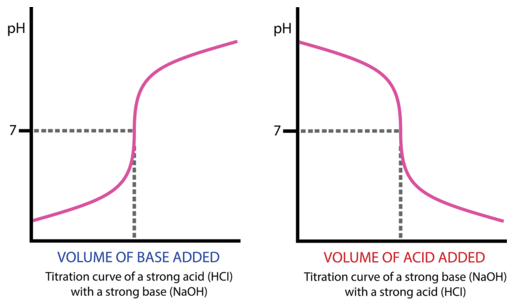
\includegraphics[width=10cm]{ph_curves}
            \caption{Titration Curves}
            \end{center}
    \end{figure}

    \section{Electrochemistry}

    \begin{description}
        \item[oxidation] involves the loss of electrons
        \item[reduction] involves the gain of electrons
        \item[redox] is the term used when describing oxidation and reduction in a reaction  
    \end{description}

    \subsection{Oxidation Numbers}

    \begin{center}
        \begin{tabular}{l | c}
            Elements by itself & 0 \\
            Group 1 & always +1 \\
            Group 2 & always +2 \\
            Halogens (Group 7) & usually -1, + with \ce{O2} \\
            Monoatomic ion & ion charge \\
            Hydrogen (\ce{H2}) & +1 with nonmetals, -1 with metals \\
            Oxygen (\ce{O2}) & usually -2, -1 in peroxide (\ce{H2O2}) \\
            Fluorine (\ce{F2}) & always -1
        \end{tabular}
        \newpage
        Sum of ON's for a neutral compound = 0 \\
        Sum of ON's for a polyatomic ion = ion charge
    \end{center}

    \subsection{Identifying Redox Reactions}
    Some helpful mnemonics: LEO the lion says GER and OILRIG
    \begin{description}
        \item[LEO] Lose electrons is oxidation
        \item[GER] Gain electrons is reduction
        \item[OIL] Oxidation is lost
        \item[RIG] Reduction is gain   
    \end{description}

    \subsection{Balancing Redox Equations}
    The oxidation of \ce{Fe^{+2}} to \ce{Fe^{+3}} by \ce{Cr2O7^{2-}} in acid solution.
    \begin{center}
        \ce{Fe^{+2} -> Fe^{+3} + e^{-}}
    \end{center}

    1. Write the unbalanced equation for the reaction in ionic form.
    \begin{center}
        \ce{Fe^{2+} + Cr2O7^{2-} -> Fe^{3+} + Cr^{3+}}
    \end{center}
    
    2. Separate the equation into two half reactions.
    \begin{center}
        \begin{tabular}{l c}
            \textbf{Oxidation} & \ce{Fe^{2+} -> Fe^{3+}} \\
            \textbf{Reduction} & \ce{Cr2O7^{2-} -> Cr^{3+}}
        \end{tabular}
    \end{center}

    3. Balance the atoms other than O and H in each half-reaction.
    \begin{center}
        \ce{Cr2O7^{2-} -> \textbf{2} Cr^{3+}}
    \end{center}

    4. For reactions in acid, add \ce{H2O} to balance O atoms and \ce{H^{+}} to balance H atoms.
    \begin{center}
        \ce{Cr2O7^{2-} -> 2 Cr^{3+} + \textbf{\ce{7 H2O}}} \\
        \ce{\textbf{\ce{14 H^{+}}} + Cr2O7^{2-} -> 2 Cr^{3+} + 7 H2O}
    \end{center}

    5. Add electrons to one side of each half-reaction to balance the charges on the half-reaction.
    \begin{center}
        \ce{Fe^{2+} -> Fe^{3+} + 1 e^{-}} \\
        \ce{\textbf{\ce{6 e^{-}}} + 14 H^{+} + Cr2O7^{2-} -> 2 Cr^{3+} + 7 H2O}
    \end{center}

    6. Use Hess' Law to make a final balanced equation by cancelling out the electrons.
    \begin{center}
        $\boxed{\ce{6 Fe^{2+} + 14 H^{+} + Cr2O7^{-2} -> 2 Cr^{3+} + 7 H2O + 6 Fe^{+3}}}$
    \end{center}

    \subsection{Cells and Cell Potentials}
    \subsubsection{Galvanic Cells}

    \begin{figure}[h]
        \begin{center}
            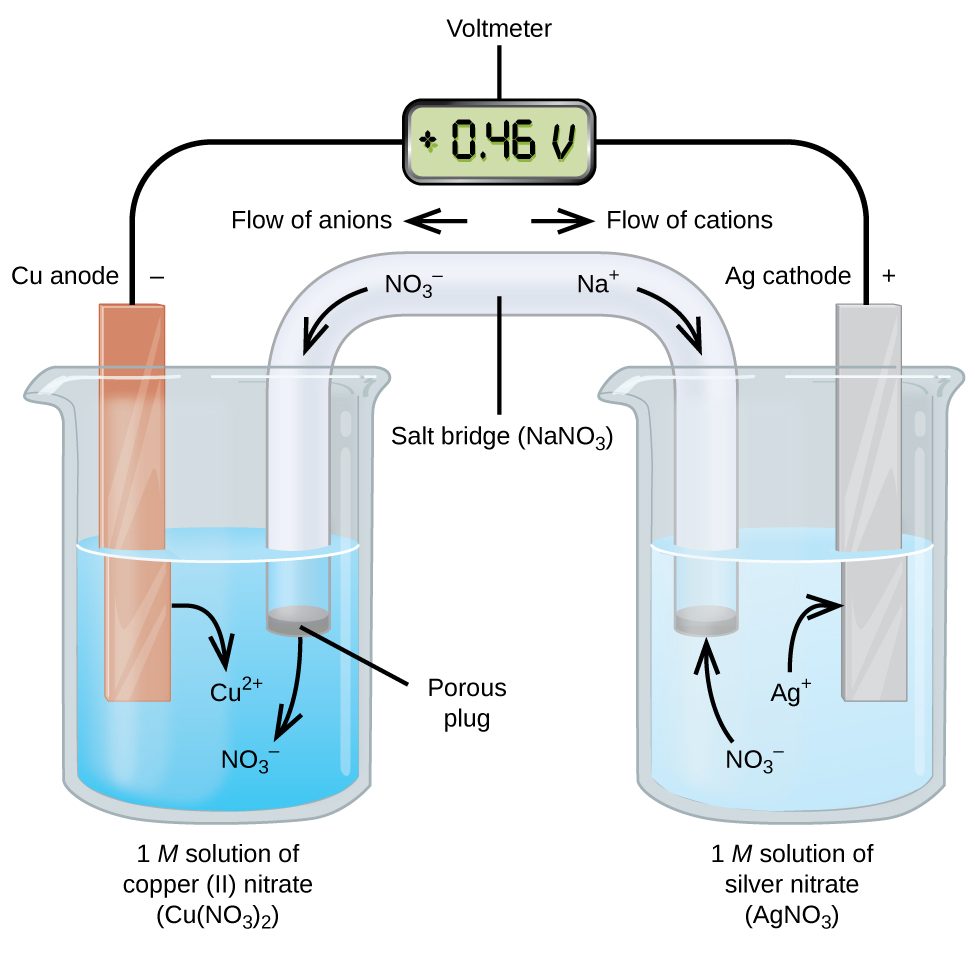
\includegraphics[width=10cm]{galvanic_cell}
            \caption{Galvanic Cell Demonstration}
        \end{center}
    \end{figure}

    \begin{description}
        \item[ANODE] where oxidation occurs (AN OX)
        \item[CATHODE] where reduction occurs (REDCAT)
    \end{description}

    The difference in electrical potential between the anode and cathode is called: \\
    $\rightarrow$ cell voltage \\
    $\rightarrow$ electromotive force (emf) \\
    $\rightarrow$ cell potential

    \subsubsection{Cell Diagram}

    \begin{center}
        \ce{Zn_{(s)} + Cu^{2+}_{(aq)} -> Cu_{(s)} + Zn^{2+}_{(aq)}} \\
        \ce{Zn_{(s)} | Zn^{2+}_{(aq)} || Cu^{2+}_{(aq)} | Cu_{(s)}}
    \end{center}

    \subsubsection{Standard Reduction Potentials}
    Standard reduction potential (E$^\circ$) is the voltage associated with a reduction reaction at an electrode when all solutes are 1 M and all gases are at 1 atm.

    \begin{equation*}
        \begin{gathered}
            \text{Standard emf (E$^\circ$ cell)} \\
            E^\circ_{cell} = E^\circ_{cathode} - E^\circ_{anode}
        \end{gathered}
    \end{equation*}

    The more positive E$^\circ$, the greater the tendency for the substance to be reduced.
\end{document}
 